\section{Tutorium 24.04.25}
\label{sec:24_04_25}
Da sich das kommende Blatt ganz um Differentialformen drehen wird, wollen wir uns die neuen Begriffe zur Differentialgeometrie aus MfP4 nochmal genauer ansehen:
\subsection{Atlanten, Orientierungen und der Satz von Stokes}
Die zentrale Definition dieses Abschnittes ist die des Atlas:
\begin{definition}{Atlas}{atlas}
Sei $M$ eine $k$-Untermannigfaltigkeit des $\R^n$. Wir nennen eine Familie
\begin{equation}
\Af := \{\phi_j: T_j \to V_j\}_{j \in J}
\end{equation}
von \textit{lokalen Parametrisierungen} mit $\cup_{j \in J} V_j =M$ einen \textbf{Atlas} von $M$
\end{definition}
Was ist die Motivation hinter dieser Definiton? Um integrieren zu können, müssen wir das Verhalten einer Funktion $f:M \to \R^n$ charakterisieren können. Das Leitmotiv der Differentialgeometrie ist es, dafür die lokale Ähnlichkeit einer MFK auszunutzen: Ist $\psi: U \to \widehat{U}$ eine Karte mit $U \subset M$ und $\widehat{U} \sub \R^k$ offen, so können wir die Stetigkeit von $f$ auf die Stetigkeit von $f \circ \phi^{-1}: \R^k \to \R^n$ mit unseren gewohnten Definitionen zurückführen. Wir bemerken aber ein Problem: Atlanten sind nicht eindeutig. Wir wollen natürlich nicht, dass unsere Definition von der Wahl eines Atlas abhängt. 
Das Problem kann man auf mehrere Arten lösen, in der Vorlesung wurde das zusammen mit der Orientierung verpackt:
\begin{definition}{Orientierung}{orientierung}
Sei $M$ eine $k$-Untermannigfaltigkeit des $\R^n$. Existiert ein Atlas $\Af$ von $M$, sodass die Kartenwechselabbildung für sich schneidende Parametrisierungen orientierungserhaltend ist, heißt $M$ \textbf{orientierbar}. Können wir weitere lokale Parametrisierungen zu $\Af$ hinzufügen, ohne eine Änderung der Orientierung zu bewirken, heißen diese \textbf{positiv orientiert}, andernfalls \textbf{negativ orientiert}.\\
Wir fassen die Orientierung einer MFK als Äquivalenzklasse auf und bezeichnen $(M,\Af)$ als \textbf{orientierte MFK}.
\end{definition}
Das war eine ganz schöne Menge, aber jetzt haben wir, was wir wollten: Eine MFK ist entweder nicht orientierbar, oder es gibt genau zwei Orientierungen bzw. Äquivalenzklassen von Atlanten auf $M$. Im Skript wird fortan die positive Orientierung gewählt. Sind die lokalen Parametrisierungen von Klasse $\cC^\infty$, nennt man $\Af$ auch glatte Struktur auf $M$.\footnote{Wer diese Definition über Äquivalenzklassen nicht so hilfreich findet, kann auch mit \textbf{maximalen Atlanten} arbeiten: Ein Atlas $\Af$ heißt \textbf{maximal}, wenn er nicht die echte Teilmenge irgendeines anderen Atlas ist.}\\
Wir wollen nun Orientierungen auf $n-1$-dimensionale Hyperflächen ausweiten.
\begin{definition}{Orientierung des Tangentialraums}{orienttang}
Sei $(M, \Af)$ eine orientierte $k$-UMF des $\R^n$ mit positiv orientierter lokaler Parametrisierung $\phi$. Für jedes $p \in M$ ist 
\begin{equation}
(\partial_1 \phi_p, \dots, \partial_k \phi_p)
\end{equation}
eine positiv orientierte Basis von $T_pM$. Die Orientierung aller weiteren Basen wird relativ dazu festgesetzt.
\end{definition}
Für eine Hyperfläche $M \sub \R^{n\geq 2}$ mit Standardorientierung erhalten wir so ein bezüglich $\Af$ positiv orientiertes \textbf{Einheitsnormalenfeld} auf $M$: Dies ist ein stetiges Vektorfeld $\nu: M \to \R^n$, sodass für alle $p \in M$ $\nu(p)$ ein Einheitsnormalenvektor von $M$ ist und gilt: Ist $(v_1, \dots, v_{n-1})$ eine positiv orientierte Basis von $T_pM$, so ist $(\nu(p), v_1, \dots, v_{n-1})$ eine positiv orientierte Basis des $\R^n$. Die wahre Erkenntnis ist dabei:
\begin{satz}{Orientierung durch Einheitsnormalenfelder}{orientierungvektor}
Sei $M \sub \R^n$ eine Hyperfläche. Ist $M$ orientiert, so existiert ein positiv orientiertes Einheitsnormalenfeld. Existiert umkehrt ein Einheitsnormalenfeld auf $M$, so definiert dieses eine Orientierung der Hyperfläche.
\end{satz}
Das hilft uns schon einmal in der Vorstellung, wenn man bedenkt, dass Einheitsnormalenfelder für $2$-Mannigfaltigkeiten recht anschaulich sind. Darüber hinaus lässt sich so auch der Rand $\partial M$ einer MFK $M$ orientieren, indem man randadaptierte Parametrisierungen mit einheitlicher Orientierung auf den Rand einschränkt.
\begin{beispiel}
Betrachte das Möbiusband $M \sub \R^3$ und die $2$-Sphäre $\S^2 \sub \R^3$. Beide sind $2$-Mannigfaltigkeiten des $\R^3$. Man betrachte folgendes Bild:\\
\begin{center}
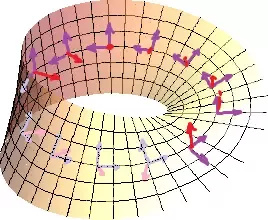
\includegraphics[scale=.3]{figures/mobius.png} 
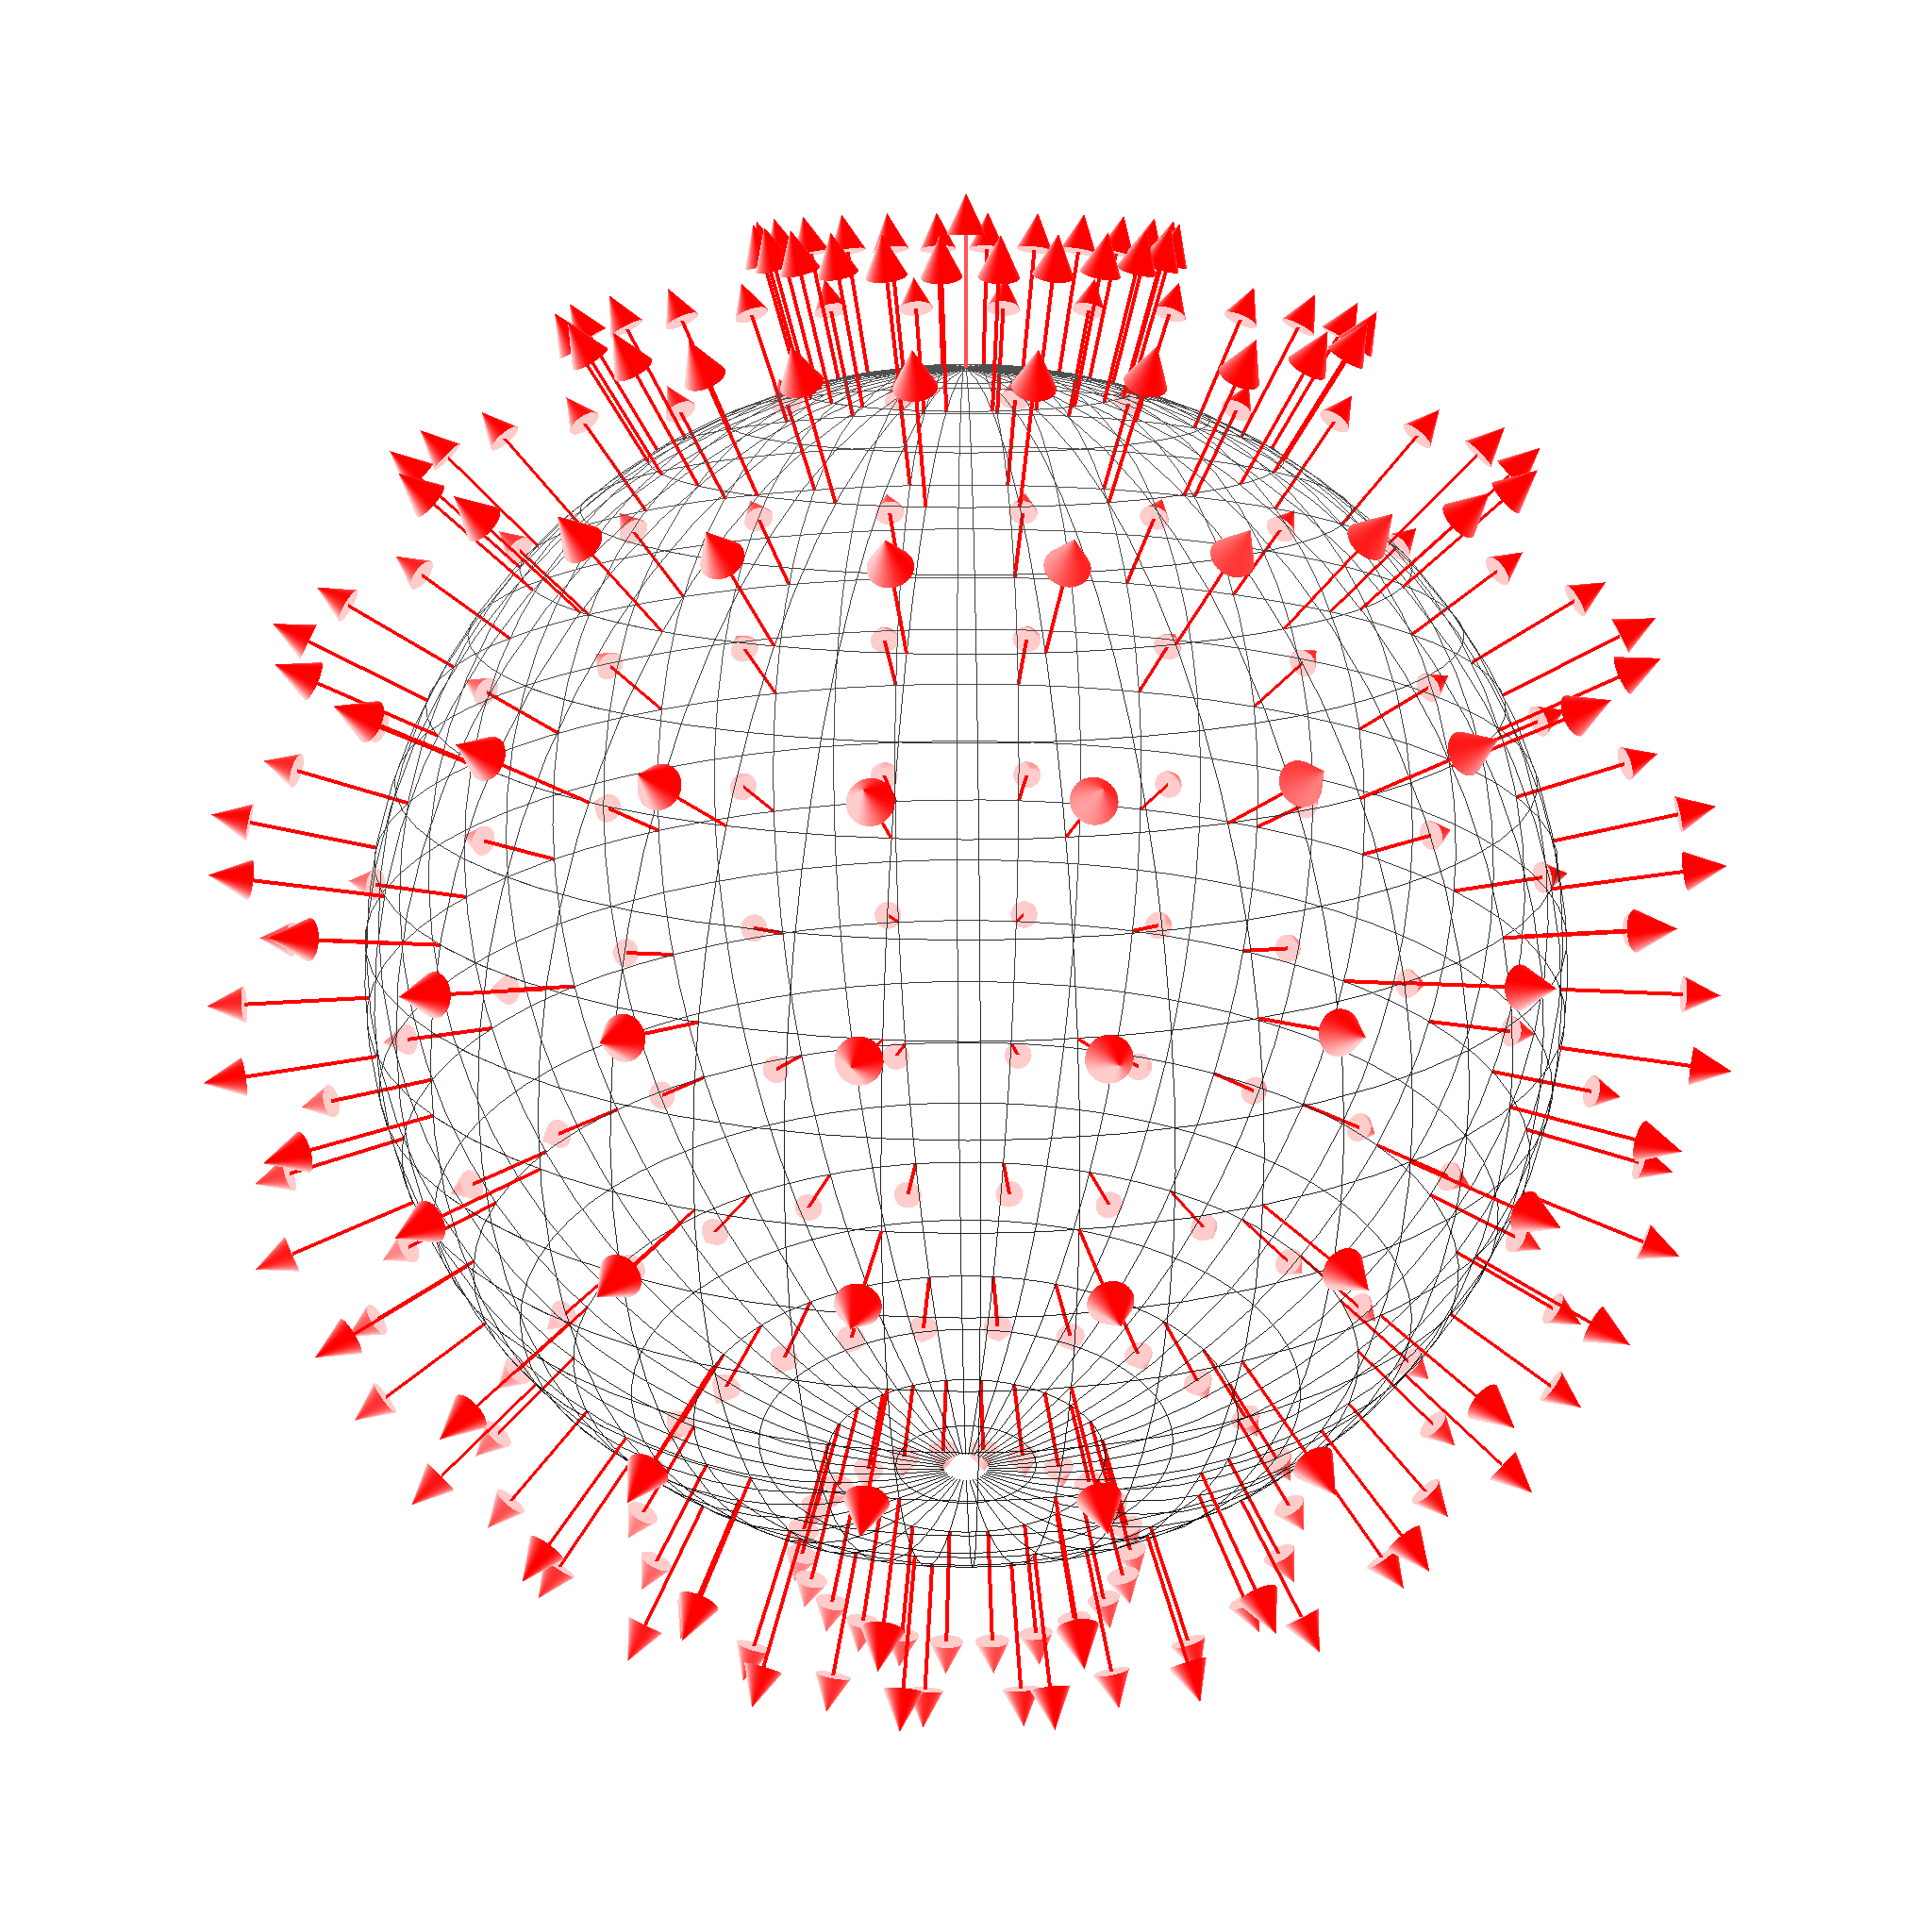
\includegraphics[scale=.05]{figures/sphere.png}
\end{center}
Erkennbar ist, dass sich das Möbiusband nicht orientieren lässt, während die Sphäre durch das Vektorfeld mit $\|v\|=1$ bereits positiv orientiert ist.
\end{beispiel}
Wir haben also jetzt alle Werkzeuge, um Integration auf der gesamten (Unter-)Mannigfaltigkeit über lokale Parametrisierungen zu verstehen. Ziel ist, eine stetige $k$-Form auf $U \sub \R^n$ über eine Teilmenge $A \sub M$ einer orientierten $k$-Untermannigfaltigkeit zu integrieren. Gibt es eine einzelne Parametrisierung $\phi: T \to V \sub M$ mit $A \sub V$, so definieren wir Integration über $A$ durch
\begin{equation}
\int_{(A, \Af)} \omega := \int_{\phi^{-1}(A)} \phi^\ast \omega.
\end{equation}
Andernfalls sei
\begin{equation}
\left( \phi_j: T_j \to V_j \sub M \right)_{j \in J}
\end{equation}
eine endliche Familie von lokalen Parametrisierungen mit $A \sub \cup_{j \in J} V_j$. Wir nehmen uns eine der Überdeckung $(V_j)_j$ untergeordnete Partition der Eins
\begin{equation}
\alpha_j: \bigcup_{l \in J} V_l \to \R
\end{equation}
her und teilen $A$ gewissermaßen auf die Träger der Partition der Eins auf mit $A_j := A \cap \supp(\alpha_j) \sub V_j$ . Jetzt können wir endlich integrieren: $\omega$ heißt \textit{integrierbar über} $A$, falls $\omega$ über alle $A_j$ integrierbar ist. Dann setzen wir
\begin{equation}
\int_{(A, \Af)} \omega := \sum_{j=1}^m \int_{\phi_j^{-1}(A_j)} (\alpha_j \circ \phi_j) \cdot (\phi_j^\ast \omega),
\end{equation}
zerstückeln das Integral also über die Partitionsmengen. Mit diesem Verständnis springen wir dann auch direkt zu einem der schönsten Sätze:
\begin{theorem}{Stokesscher Integralsatz}{stokes}
Sei $U \sub \R^n$ offen und $\omega$ eine glatte $(k-1)$-Form auf $U$ mit $k \geq 2$. Sei $M \sub U$ eine $k$-Untermannigfaltigkeit. Für jedes Kompaktum $A \sub M$ mit glattem Rand $\partial A$, orientiert durch $M$, gilt:
\begin{equation}
\int_A d\omega = \int_{\partial A} \omega.
\end{equation}
\end{theorem}
Daraus erhalten wir eine schöne Aussage für unberandete, kompakte Mannigfaltigkeiten $M$. Ist $M \sub U$ wie oben, aber $\partial M = \emptyset$, so erhalten wir direkt
\begin{equation}
\int_M d\omega = \int_\emptyset \omega = 0.
\end{equation}
Es gibt noch viele weitere schöne Aussagen, die daraus folgen und einen expliziten Zusammenhang zu exakten Differentialformen aufzeigen. Tatsächlich bekommen wir dadurch konkrete Äquivalenzen, die Exaktheit und Geschlossenheit mit bestimmten Integralen gleichsetzen. Für die Interessierten: Dies findet man unter den Stichworten \textit{De Rahm-Kohomologie} und \textit{De Rahm-Theorem}.